\documentclass[10pt, table, dvipsnames,xcdraw,handout]{beamer}
\usetheme[progressbar=frametitle]{metropolis}
\usepackage{appendixnumberbeamer}
\usetikzlibrary{arrows.meta, positioning, quotes}
\usepackage[shortlabels]{enumitem}
\usepackage{xcolor}
\usepackage{mathtools}
\usepackage{dsfont}

\usepackage{caption}


\usepackage{cancel}

\newcommand\hcancel[2][black]{\setbox0=\hbox{$#2$}%
\rlap{\raisebox{.45\ht0}{\textcolor{#1}{\rule{\wd0}{1pt}}}}#2} 


\usepackage{booktabs}
\usepackage[scale=2]{ccicons}

\usepackage{pgfplots}
\usepgfplotslibrary{dateplot}

\usepackage{xspace}
\newcommand{\themename}{\textbf{\textsc{metropolis}}\xspace}
\newcommand{\cb}{\cellcolor{blue!25}}


% Notation:
\newcommand{\cT}{\ensuremath{\mathcal{T}}}
\newcommand{\cD}{\ensuremath{\mathcal{D}}}
\newcommand{\cX}{\ensuremath{\mathcal{X}}}
\newcommand{\cY}{\ensuremath{\mathcal{Y}}}
\newcommand{\cZ}{\ensuremath{\mathcal{Z}}}
\newcommand{\cH}{\ensuremath{\mathcal{H}}}
\newcommand{\cG}{\ensuremath{\mathcal{G}}}

\newcommand{\bR}{\ensuremath{\mathbb{R}}}
\newcommand{\bN}{\ensuremath{\mathbb{N}}}
\newcommand{\bP}{\ensuremath{\mathbb{P}}}
\newcommand{\bT}{\ensuremath{\mathbb{T}}}
\newcommand{\bL}{\ensuremath{\mathbb{L}}}

\newcommand{\bfX}{\ensuremath{\mathbf{X}}}
\newcommand{\bfY}{\ensuremath{\mathbf{Y}}}
\newcommand{\bfy}{\ensuremath{\mathbf{y}}}
\newcommand{\bfD}{\ensuremath{\mathbf{D}}}

\def\layersep{2.5cm}

% Tikz seys
\tikzset{cross/.style={cross out, draw, 
         minimum size=2*(#1-\pgflinewidth), 
         inner sep=0pt, outer sep=0pt}}

\title{Machine Learning I}
\subtitle{Lecture 15: Cluster Analysis Part I}
% \date{\today}
\date{}
\author{Nathaniel Bade}
\institute{Northeastern University Department of Mathematics}
% \titlegraphic{\hfill\includegraphics[height=1.5cm]{logo.pdf}}

\begin{document}

\maketitle

\begin{frame}{Table of contents}
  \setbeamertemplate{section in toc}[sections numbered]
  \tableofcontents[hideallsubsections]
\end{frame}


%%%%%%%%%%%%%% Slidshow Start %%%%%%%%%%%%%% 


%Notes: 4 kinds of clusering: Centroid based/kmeans, connecctivity based, density based, distribution based. 
%
% What metrics can we use to evalaute scattering? (internal) Scatter crieteria, silloett coeffcient, (external) mutial information, 
% 
%
% Association rules and merket basket analysis. 
%
%
%
%


\section{Cluster Analysis}

\begin{frame}[fragile]{Cluster Analysis}
  \begin{minipage}[t][0.5\textheight][t]{\textwidth}
	\centering \includegraphics[height=0.5\textheight]{L15ClusterIntro.png} 
  \end{minipage}
  \vfill
\begin{minipage}[t][0.5\textheight][t]{\textwidth}
Clustering is one of the most widely used techniques in exploratory data analysis. Clustering is the task of organizing data into groups so that ``similar" objects end up in the same \textbf{cluster} and ``different'' objects end up in different clusters. 
\end{minipage}
\end{frame}



\begin{frame}[fragile]{Cluster Analysis}
  \begin{minipage}[t][0.5\textheight][t]{\textwidth}
	\centering \includegraphics[height=0.5\textheight]{L15ClusterIntro2.png} 
  \end{minipage}
  \vfill
\begin{minipage}[t][0.5\textheight][t]{\textwidth}
The basic problem for clustering is a problem for all unsupervised learning: the problem of ground truth. Since there are no labels from which to learn what possible clusters might look like, we have to make assumptions about how the data are grouped. 
\end{minipage}
\end{frame}



\begin{frame}[fragile]{Cluster Analysis}
  \begin{minipage}[t][0.5\textheight][t]{\textwidth}
	\centering \includegraphics[height=0.5\textheight]{L15ClusterIntro3.png} 
  \end{minipage}
  \vfill
\begin{minipage}[t][0.5\textheight][t]{\textwidth}
The basic problem for clustering is a problem for all unsupervised learning: the problem of ground truth. Since there are no labels from which to learn what possible clusters might look like, we have to make assumptions about how the data are grouped. \pause

A clustering algorithm that emphasizes similarly labeling close by points will not be as aware of the total distance in feature space, while a method that emphasizes not having far away points will ignore local information. 
\end{minipage}
\end{frame}



\begin{frame}[fragile]{Clustering Paradigms}
There are five basic kinds of clustering paradigms: 
\begin{itemize}
\item[] \textbf{Centroid} based clustering is governed by overall distance to closest centroid.\pause
\item[] \textbf{Hierarchical} clustering build nested clusters by merging or splitting, forming a cluster \textbf{dendrogram}.\pause
\item[] \textbf{Density} based methods are determined by contiguous regions with density above some threshold.\pause
\item[] \textbf{Spectral} clustering decomposes the similarity graph $d(x_i,x_j)$ as in factor analysis and PCA.\pause
\item[] \textbf{Distribution models/mixing models} assume clusters provide a underlying distribution on the domain.
\end{itemize}
\end{frame}

\begin{frame}[fragile]{Centroid Based Clustering}
  \begin{minipage}[t][0.5\textheight][t]{\textwidth}
	\centering \includegraphics[height=0.5\textheight]{L15Kmeans1.png}\hspace{1em}\includegraphics[height=0.5\textheight]{L15Kmeans2.png} 
  \end{minipage}
  \vfill
\begin{minipage}[t][0.5\textheight][t]{\textwidth}
In centroid based clustering, clusters are determined by distance from a centroid $\mu_i$, under a metric $d(x,y)$ of similarity matrix $D$. \pause Examples include \texttt{$k$-means}, \texttt{$k$-mediods}, and the \texttt{meanshift} algorithm. 
\end{minipage}
\end{frame}


\begin{frame}[fragile]{Hierarchical Clustering}
  \begin{minipage}[t][0.5\textheight][t]{\textwidth}
	\centering \includegraphics[height=0.6\textheight]{L15Linkage.png}\hspace{3em}\includegraphics[height=0.6\textheight]{L15Linkage2.png} 
  \end{minipage}
  \vfill
\begin{minipage}[t][0.4\textheight][t]{\textwidth}
In hierarchical (connectivity, linkage) clustering, nested clusters are formed using greedy algorithms but either merging or splitting sets. \pause Algorithms include \texttt{Ward} and \texttt{AgglomerativeClustering}. 
\end{minipage}
\end{frame}


\begin{frame}[fragile]{Density Based Clustering}
  \begin{minipage}[t][0.5\textheight][t]{\textwidth}
	\centering \includegraphics[height=0.5\textheight]{L15Cont1.png}\hspace{1em}\includegraphics[height=0.5\textheight]{L15Cont2.png} 
  \end{minipage}
  \vfill
\begin{minipage}[t][0.5\textheight][t]{\textwidth}
Density based clustering algorithms determine regions by applying a local density threshold (with a dynamically determined or fixed density) and then extracting the connected regions. \pause Algorithms like DBSCAN on the right assume clusters are of similar density and have trouble separating nearby clusters. Algorithms like OPTICS improve upon this but are not currently implemented. 
\end{minipage}
\end{frame}


\begin{frame}[fragile]{Spectral Clustering}
  \begin{minipage}[t][0.5\textheight][t]{\textwidth}
	\centering \includegraphics[height=0.5\textheight]{L15Spetral.png}
  \end{minipage}
  \vfill
\begin{minipage}[t][0.5\textheight][t]{\textwidth}
Spectral clustering forms a similarity matrix $S_{ij}$ where each entry encode the similarity between datapoints $i$ and $j$. We then project onto the first $k$ eigenvectors of $S_{ij}$ and perform the clustering there. \pause Equivalently, we can construct a similarity graph and thing of pruning away low relevance connections until the graph disconnects. Sci-kit learn implements this as SpectralClustering.
\end{minipage}
\end{frame}



\begin{frame}[fragile]{Distribution Based Clustering}
  \begin{minipage}[t][0.5\textheight][t]{\textwidth}
	\centering \includegraphics[height=0.5\textheight]{L15Dist1.png}\hspace{1em}\includegraphics[height=0.5\textheight]{L15Dist2.png} 
  \end{minipage}
  \vfill
\begin{minipage}[t][0.5\textheight][t]{\textwidth}
Distribution based, or mixing models, try to fit an underlying distribution to the data, often using maximum likelihood estimation. This is implemented in sci-kit learn as GaussianMixture.\pause
\end{minipage}
\end{frame}



\begin{frame}[fragile]
  \begin{minipage}[t][0.8\textheight][t]{\textwidth}
	\centering \includegraphics[height=0.8\textheight]{L15ClusterComp2.png}
  \end{minipage}
  \vfill
\begin{minipage}[t][0.2\textheight][t]{\textwidth}
Sci-kit learn's clustering algorithms compared: \url{https://scikit-learn.org/stable/modules/clustering.html}
\end{minipage}
\end{frame}







\section{K-Means Clusters}
\begin{frame}[fragile]{K-Means Clusters}
  \begin{minipage}[t][0.5\textheight][t]{\textwidth}
	\centering \includegraphics[height=0.5\textheight]{L15Kmeans1.png}\hspace{1em}\includegraphics[height=0.5\textheight]{L15Kmeans2.png} 
  \end{minipage}
  \vfill
\begin{minipage}[t][0.5\textheight][t]{\textwidth}
The K-means clustering algorithm constructs $K$ clusters $C_j$ by their proximity to a centroid $\mu_j$. The algorithm attempts to minimize the distance to the centroid $\mu_j$:
$$
L(\mu) = \sum_{j=1}^K\sum_{x_i\in C_=j}  ||x_i - \mu_j||^2\,.
$$
\end{minipage}
\end{frame}


\begin{frame}[fragile]{K-Means Clusters}
  \begin{minipage}[t][0.5\textheight][t]{\textwidth}
	\centering \includegraphics[height=0.5\textheight]{L15Kmeans1.png}\hspace{1em}\includegraphics[height=0.5\textheight]{L15Kmeans2.png} 
  \end{minipage}
  \vfill
\begin{minipage}[t][0.5\textheight][t]{\textwidth}
For $d$ given by the Euclidean distance, one can see that this is roughly equivalent to minimizing the \textbf{within group scatter}:
$$
W(C) = \sum_{j=1}^K\sum_{x_i,x_{i'}\in C_=j} ||x_{i}-x_{i'}||^2 \pause = \sum_{j=1}^KN_j\sum_{x_i\in C_j} ||x_i - \mu_j||^2\,.
$$
\end{minipage}
\end{frame}



\begin{frame}[fragile]{K-Means Algorithm}
A brute force search is NP hard. However, there exists an iterative procedure to find a local minimum. \pause Since 
$$
\text{argmin}_\mu \,\sum_{i\in S}||x_i - \mu||^2 = \bar x_S\,,
$$
where $\bar{x}_S$ is the mean of the $x$'s in $S$, we can solve the enlarged problem by the following algorithm:\pause\newline

Initialize $\mu_j$ to random values. Then
\begin{itemize}
\item[] For each $j$, set $C_j^{(t)} = \{x_i\in \mathcal{X}:\, j = \text{argmin}_k ||x_i-\mu^{(t-1)}_k||^2\}$. \pause
\item[] For each $j$, update $\mu_j^{(t)} = \bar x_{C_j^{(t)}}$\,. \pause
\item[] Repeat until convergence. 
\end{itemize}
\end{frame}



\begin{frame}[fragile]{K-Means Algorithm}
\textbf{Lemma:} The K-Means algorithm is non-increasing.\newline\pause

\textbf{Proof:}
At step $t$, let $C^{(t-1)}_j$ be the previous clusters and $\mu_{j}^{(t-1)}$ the previous centroids. The total cluster variance
$$
W(C^{(t-1)},\mu^{(t-1)})  = \sum_{j=1}^KN_j\sum_{x_i\in C_j^{(t-1)}} ||x_i - \mu_j||^2
$$
is minimized by setting the means at time step $t$ to $\mu_j^{(t)} = \bar x_{C_j^{(t-1)}}$. Therefore $W(C^{(t-1)},\mu^{(t-1)}) \geq W(C^{(t-1)},\mu^{(t)})$.

\pause But, given this current set of means $\mu_j^{(t)}$, $W(C^{(t)})$ will be minimized by setting
$$
C_j^{(t)} = \{x\in \mathcal{X}:\, i = \text{argmin}_j ||x-\mu||^2\}\,.
$$
Therefore $W(C^{(t-1)},\mu^{(t)}) \geq W(C^{(t)},\mu^{(t)})$.

\end{frame}



\begin{frame}[fragile]{Example: }
  \begin{minipage}[t][0.6\textheight][t]{\textwidth}
	\centering \includegraphics[height=0.6\textheight]{L15KMeanSteps.png} 
  \end{minipage}
  \vfill
\begin{minipage}[t][0.4\textheight][t]{\textwidth}
The efficiency of the algorithm come from it's greedy nature. Note in the example above that we have probably not found the global minimum, but that the clustering has found reasonable divisions given three labels. 
\end{minipage}
\end{frame}



\section{Practical Considerations for $k$-means}




\begin{frame}[fragile]{Practical Issues: Initialization}
\textbf{Question:} Assume we initialize the algorithm by picking the cluster centers at random from the dataset. How bad can our initialization scheme be? Can you come up with a set of 4 point and an initialization such that the $K$-means algorithm never finds the global minimum?\pause

\vspace{12em}
In practice though does this really happen?
\end{frame}







\begin{frame}[fragile]{Practical Issues: Initialization}
  \begin{minipage}[t][0.5\textheight][t]{\textwidth}
	\centering \includegraphics[height=0.5\textheight]{L14Inintilization.png} 
  \end{minipage}
  \vfill
\begin{minipage}[t][0.5\textheight][t]{\textwidth}
Absolutely. For example, the initialization given to the clusters leads to a highly non-optimal clustering. 
\end{minipage}
\end{frame}





\begin{frame}[fragile]{Random Initialization}
  \begin{minipage}[t][0.5\textheight][t]{\textwidth}
	\centering \includegraphics[height=0.5\textheight]{L14Inintilization2.png} 
  \end{minipage}
  \vfill
\begin{minipage}[t][0.5\textheight][t]{\textwidth}
\textbf{Question:} How likely is such a clustering in practice? Given 4 clusters arranged as above (with equal numbers of points per cluster), what is the probability of randomly choosing a bad cluster?
\end{minipage}
\end{frame}









\begin{frame}[fragile]{Practical Issues: Initialization}
\textbf{Initialization} is probably the greatest difficulty in most greedy algorithms. \pause For example, assume we initialize by setting $\mu_j$ to be randomly selected data points $x_j$. 

If the data has $K$ clusters, each of size $N/K$, then the probability of randomly selecting a point from each cluster is
$$
\frac{K-1}{K}\frac{K-2}{K}\ldots \frac{1}{K}\pause = \frac{K!}{K^K} \pause \leq \left( \frac12\right)^{\frac K2}\,.
$$\pause
So we will almost always have bad initial centroids for $K$ large. \pause

To get better results: Always take multiple randomized starts and consider ensambling them. Initialize with bottom up hierarchical methods. Alternatively, select more than $k$ points and only keep the most widely separated. Finally, we can use a different initialization scheme. 
\end{frame}







\begin{frame}[fragile]{Furthest Point Initialization}
  \begin{minipage}[t][0.5\textheight][t]{\textwidth}
	\centering \includegraphics[height=0.5\textheight]{L14Inintilization3.png} 
  \end{minipage}
  \vfill
\begin{minipage}[t][0.5\textheight][t]{\textwidth}
\textbf{Furthest point} initialization works better for Gaussian clusters. Pick an initial $\mu^{(0)}_1$ at random. Then for $\mu^{(0)}_j$, $j=2,\ldots, k$, pick $\mu^{(0)}_j$ to be the farthest point away from $\mu^{(0)}_1$ though $\mu^{(0)}_{j-1}$\,.\pause
\end{minipage}
\end{frame}







\begin{frame}[fragile]{Furthest Point Initialization}
  \begin{minipage}[t][0.5\textheight][t]{\textwidth}
	\centering \includegraphics[height=0.5\textheight]{L14Inintilization4.png} 
  \end{minipage}
  \vfill
\begin{minipage}[t][0.5\textheight][t]{\textwidth}
However, it is very sensitive to outliers, as for example in the three clusters above. 
\end{minipage}
\end{frame}









\begin{frame}[fragile]{$k$ means++}
A third popular initialization scheme was proposed in 2007 that interpolates between $k$-means and furthest point initialization. 

Pick a point $\mu^{(0)}_{1}$ at random. Assume we've picked centers $\mu^{(0)}_{1},\ldots, \mu^{(0)}_{j-1}$. For each point $x$, let $D(x)$ be the distance from $x$ to the closest center. Define a distribution on the $x_i$ by
$$
\mathcal{D}(x_i) = \frac{D^\alpha(x_j)}{\sum_j D^\alpha(x_j)}\,.
$$\pause
If $\alpha=0$, then all points are equally likely as in $k$-means. If $\alpha = \infty$, then $\mathcal{D}(x_i) = \text{argmax}_i(D(x_i))$ as in furthest point initialization. \pause

For $k$-means++, we set the hyperparameter $\alpha = 2$.

\end{frame}





\begin{frame}[fragile]{$k$ means++}
$k$-means++ comes with some nice theoretical guarantees: 
\begin{itemize}
\item The expected value of the optimization function when initialized with $k$-means ++ is $O(\log k)$ times the optimal value. 

\item A slightly modified version is an $O(1)$ approximation if the data is \emph{nicely clusterable} with $k$ clusters.
\end{itemize} 

Here, a nicely clusterable point set $X$ is on for which increasing the number of clusters by 1 decreases the total error by a roughly fixed amount. Concretely,
$$
W_k(X) \leq \epsilon^2 W_{k-1}(X) 
$$
in expected value.\pause $k$-means++ has computational issues on large, high dimensional datasets, but has been demonstrated as an effective classifier for pictures.\hyperlink{reference}{\beamergotobutton{$^1$}}
\end{frame}








\begin{frame}[fragile]{Practical Issues: Choosing $K$}
  \begin{minipage}[t][0.5\textheight][t]{\textwidth}
	\centering \includegraphics[height=0.5\textheight]{L15MSE.png} 
  \end{minipage}
  \vfill
\begin{minipage}[t][0.5\textheight][t]{\textwidth}
The choice of $K$ is the other main practical issue in $K$-means clustering. A common criteria is to compute the clustering for many $K$, plot them, and set $K$ to be just larger than the steepest ``elbow,'' or ``kink.'' \pause In the example above, we might choose $K = 4$ or $K = 7$.
\end{minipage}

\end{frame}


\begin{frame}[fragile]{Practical Issues: Choosing $K$}
  \begin{minipage}[t][0.5\textheight][t]{\textwidth}
	\centering \includegraphics[height=0.5\textheight]{L15GAP.png} 
  \end{minipage}
  \vfill
\begin{minipage}[t][0.5\textheight][t]{\textwidth}
There are various purposed automatic methods for this, including the \textbf{gap statistic} which attempts to makes the idea of a ``elbow'' precise by comparing the within cluster dissimilarity $W_i$ to the expected dissimilarity for a uniform distribution over a rectangle containing the data. 
\end{minipage}

\end{frame}




\begin{frame}[fragile]{Practical Issues: Size and Density}
  \begin{minipage}[t][0.5\textheight][t]{\textwidth}
	\centering \includegraphics[width=\textwidth]{L15Errors.png} 
  \end{minipage}
  \vfill
\begin{minipage}[t][0.5\textheight][t]{\textwidth}
$K$-means can be thrown off by varying size and density. The squared term in the loss penalizes relatively large clusters, while the sum over all points weights denser patches more heavily. 
\end{minipage}

\end{frame}



\begin{frame}[fragile]{Practical Issues: Size and Density}
  \begin{minipage}[t][0.5\textheight][t]{\textwidth}
	\centering \includegraphics[width=\textwidth]{L15ClusterComp3.png} 
  \end{minipage}
  \vfill
\begin{minipage}[t][0.5\textheight][t]{\textwidth}
Finally, $K$-means is a centroid based method and so is optimized on position in space, not position relative to other points. This means that contiguous clusters with a less symmetric geometry will not be found. \pause By optimizing over balls, $K$-means is forming linear decision boundaries, and cannot find other kinds of boundaries without being embedded in a higher dimensional space. 
\end{minipage}
\end{frame}




\begin{frame}[fragile]{$k$-Means Review}
\textbf{Review Questions:}

What kinds of datasets does $k$-means work well on? What kind does it work poorly on. 

What is the difference between the three initializations? When should you use one or the other?  

Assume you perform a clustering on an unknown dataset. For each initialization, what would be evidence that you had picked the wrong initialization?

What is the gap statistic, and what is it used for? Can you think of a better measure?
\end{frame}













\section{Example: Gene Expression Clustering}
\begin{frame}[fragile]{Example: Gene Expression Clustering}
  \begin{minipage}[t][0.5\textheight][t]{\textwidth}
	\centering \includegraphics[height=0.5\textheight]{L15GeneExpression.png} 
  \end{minipage}
  \vfill
\begin{minipage}[t][0.5\textheight][t]{\textwidth}
The dataset Multiclass Cancer Diagnosis Using Tumor Gene Expression Signatures lists 16063 genes for 144 patients with one of 14 types of cancer: breast, prostate, lung, collerectal, lymphoma, bladder, melanoma, uterus, leukemia, renal, pancreas, ovary, meso, and cns.

\end{minipage}
\end{frame}


\begin{frame}[fragile]{Example: Gene Expression Clustering}
  \begin{minipage}[t][0.5\textheight][t]{\textwidth}
	\centering \includegraphics[height=0.5\textheight]{L15MicroArray.png} 
  \end{minipage}
  \vfill
\begin{minipage}[t][0.5\textheight][t]{\textwidth}
In the above we see a similar DNA microarray colored by expression levels. On the left we see an attempt at hierarchical clustering that we will expand on next week. \pause

The goal is to see if certain genes tend to express certain types of cancers. We could of course treat this as a supervised learning problem, but it would be a much stronger result if the clusters can be learned unsupervised. 
\end{minipage}
\end{frame}




\begin{frame}[fragile]{Example: $K=3$}
  \begin{minipage}[t][0.5\textheight][t]{\textwidth}
	\centering \includegraphics[height=0.5\textheight]{L15GeneExpr1.png} 
  \end{minipage}
  \vfill
\begin{minipage}[t][0.5\textheight][t]{\textwidth}
As a first pass we use $K$-Means clustering with $K=3$. Notice that Cluster 1, accounts for almost all of the cases of leukemia, while lymphoma and cns are localized in cluster 2. \pause

We are certainly seeing some differentiation between the cancers based solely on gene clustering, but so far we've just picked an arbitrary $K$, not even corresponding to  our 14 labels. 
\end{minipage}
\end{frame}






\begin{frame}[fragile]{Example: $K$ vs MSE}
  \begin{minipage}[t][0.5\textheight][t]{\textwidth}
	\centering \includegraphics[height=0.5\textheight]{L15MSE2.png} 
  \end{minipage}
  \vfill
\begin{minipage}[t][0.5\textheight][t]{\textwidth}
We plot the mean squared error vs the number of clusters $K$. The plot has a couple of elbows, the most significant being the ones at 4 and in the 6, 7 range. There is a bump at 12, but this may be due some other error. It isn't stable under multiple runs and is probably the result of over fitting.  
\end{minipage}
\end{frame}




\begin{frame}[fragile]{Example: $K$ vs MSE}
  \begin{minipage}[t][0.5\textheight][t]{\textwidth}
	\centering \includegraphics[height=0.5\textheight]{L15FourClust.png} 
  \end{minipage}
  \vfill
\begin{minipage}[t][0.5\textheight][t]{\textwidth}
The histogram cluster labels for 4 clusters is very promising. We see at least leukemia and cns isolated with lymphoma expressing strongly in cluster 2. 
\end{minipage}
\end{frame}

\begin{frame}[fragile]{Example: $K$ vs MSE}
  \begin{minipage}[t][0.5\textheight][t]{\textwidth}
	\centering \includegraphics[height=0.5\textheight]{L15FourClust2.png} 
  \end{minipage}
  \vfill
\begin{minipage}[t][0.5\textheight][t]{\textwidth}
The histogram cluster labels for 4 clusters is very promising. We see at least leukemia and cns isolated with lymphoma expressing strongly in cluster 2. Whats more this division is fairly stable across runs. 
\end{minipage}
\end{frame}




\begin{frame}[fragile]{Example: $K$ vs MSE}
  \begin{minipage}[t][0.5\textheight][t]{\textwidth}
	\centering \includegraphics[height=0.5\textheight]{L15FourClust3.png} 
  \end{minipage}
  \vfill
\begin{minipage}[t][0.5\textheight][t]{\textwidth}
Finally, initializing with $K$-means++ as in the fitting above gives almost the same clusters. 
\end{minipage}
\end{frame}


\begin{frame}[fragile]{Example: $K$ vs MSE}
  \begin{minipage}[t][0.5\textheight][t]{\textwidth}
	\centering \includegraphics[height=0.5\textheight]{L15FourClust.png} 
  \end{minipage}
  \vfill
\begin{minipage}[t][0.5\textheight][t]{\textwidth}
Concretely, lets look at the cluster vs label heatmap corresponding to our original example. 
\end{minipage}
\end{frame}




\begin{frame}[fragile]{Example: $K$ vs MSE}
  \begin{minipage}[t][0.5\textheight][t]{\textwidth}
	\centering \includegraphics[height=0.5\textheight]{L15FourClustHM.png} 
  \end{minipage}
  \vfill
\begin{minipage}[t][0.5\textheight][t]{\textwidth}
Concretely, lets look at the cluster vs label heatmap corresponding to our original example.  We see that in fact we missed something: certain cancers were over represented in the data and in fact cluster one contains 100\% of the breast, prostate, and bladder cancer.
\end{minipage}
\end{frame}




\begin{frame}[fragile]{Example: $K$ vs MSE}
  \begin{minipage}[t][0.5\textheight][t]{\textwidth}
	\centering \includegraphics[height=0.5\textheight]{L15GeneTotals.png} 
  \end{minipage}
  \vfill
\begin{minipage}[t][0.5\textheight][t]{\textwidth}
Indeed, we see that lymphoma, leukemia and cns are over represented in this dataset, which almost certainly accounts for the  clusters containing these types of cancer specifically. \pause But on the other hand it means the clusters are indeed are differential.
\end{minipage}
\end{frame}



\begin{frame}[fragile]{Example: $K$ vs MSE}
  \begin{minipage}[t][0.5\textheight][t]{\textwidth}
	\centering \includegraphics[height=0.5\textheight]{L15FourClustHM.png} 
  \end{minipage}
  \vfill
\begin{minipage}[t][0.5\textheight][t]{\textwidth}
In fact, we see seem to be seeing here is a lot of cancers expressing with a similar gene cluster profile while two cancers seem to be very different, and possibly another cluster containing melanoma, ovary and cns. 
\end{minipage}
\end{frame}



\begin{frame}[fragile]{Example: $K$ vs MSE}
  \begin{minipage}[t][0.5\textheight][t]{\textwidth}
	\centering \includegraphics[height=0.5\textheight]{L15SixCluster.png} 
  \end{minipage}
  \vfill
\begin{minipage}[t][0.5\textheight][t]{\textwidth}
For six clusters, we see even more specialization. 
\end{minipage}
\end{frame}


\begin{frame}[fragile]{Example: $K$ vs MSE}
  \begin{minipage}[t][0.5\textheight][t]{\textwidth}
	\centering \includegraphics[height=0.5\textheight]{L15FourteenClust.png} 
  \end{minipage}
  \vfill
\begin{minipage}[t][0.5\textheight][t]{\textwidth}
As a final example, lets look at the 14 cluster version. We see that while some clusters are well represented, we have not really improved on our separation for many of the cancers. 
\end{minipage}
\end{frame}



\begin{frame}[fragile]{Example: $K$ vs MSE}
  \begin{minipage}[t][0.5\textheight][t]{\textwidth}
	\centering \includegraphics[height=0.5\textheight]{L15SixClusterHM.png} 
  \end{minipage}
  \vfill
\begin{minipage}[t][0.5\textheight][t]{\textwidth}
For six clusters, we see even more specialization. The heatmap in particular shows that breast and prostate cancer are still expressing similarly, that lymphoma, cns and melanoma have different expressions than other cancers.
\end{minipage}
\end{frame}



\begin{frame}[fragile]{Example: $K$ vs MSE}
  \begin{minipage}[t][0.5\textheight][t]{\textwidth}
	\centering \includegraphics[height=0.5\textheight]{L15SixClusterHM.png} 
  \end{minipage}
  \vfill
\begin{minipage}[t][0.5\textheight][t]{\textwidth}
I would stress that all of these ``results" should be put in their proper context: they are indications that there is a connection, not evidence of one. The fact that just by clustering the features we can separate some different types of cancer is exciting, but it's the beginning of a lot of work not the end.
\end{minipage}
\end{frame}




\begin{frame}[fragile]{Example: $K$ vs MSE}
  \begin{minipage}[t][0.5\textheight][t]{\textwidth}
	\centering \includegraphics[height=0.5\textheight]{L15SixClusterHM.png} 
  \end{minipage}
  \vfill
\begin{minipage}[t][0.5\textheight][t]{\textwidth}
In fact, the data analysis isn't even done. Recall that this clustering is given by a linear decision boundary. We could now try to fit linear functions, or we could attempt to cluster using less linear methods. 
\end{minipage}
\end{frame}





\begin{frame}[fragile]{Review Questions}
\textbf{Review Questions:}

Why do we use 4/6 clusters, even though we know there are 14 labels?

Assume that the 14 clusters are in fact disconnected Gaussian balls, how many would we expect to successfully find using $K$-means with a random initialization?

Consider the 4 cluster labeling vs the 6 cluster labeling? While neither should be taken literally, together do they indicate a genetic separation between cancers, and for which cancers?

If you wanted to derive a $p$-value for the $4$-cluster fit, how could you do so?
\end{frame}








\section{Density Based Clustering}


\begin{frame}[fragile]{Density Based Clustering}
  \begin{minipage}[t][0.5\textheight][t]{\textwidth}
	\centering \includegraphics[height=0.5\textheight]{L15Cont1.png} 
  \end{minipage}
  \vfill
\begin{minipage}[t][0.5\textheight][t]{\textwidth}
In density based clustering, we try to construct continuous neighborhoods of points based on being above some threshold density. \pause For a fixed radius $r$, a point $x_i$ is considered part of a cluster if the number of points in $B_{r}(x_i) = \{x_j \,:\, ||x_i - x_j||\}$ is sufficiently large. \pause Fix $n_r$ to be the number of points required to be in a cluster. 
\end{minipage}
\end{frame}



\begin{frame}[fragile]{DBSCAN Definitions}
  \begin{minipage}[t][0.5\textheight][t]{\textwidth}
	\centering \includegraphics[height=0.5\textheight]{L15DBS.png} 
  \end{minipage}
  \vfill
\begin{minipage}[t][0.5\textheight][t]{\textwidth}
The DBSCAN algorithm classifies points a \textbf{core points} like A, \textbf{boundary points} like B and C, and \textbf{noise points} like N. \pause \newline

A core point is one for which $B_r(p)\geq n_r$. A point $q$ is \textbf{directly reachable} from $p$ if $q\in B_r(p)$. \pause If a point $q$ is directly reachable from a core point then it is a boundary point. \pause If a point is not directly reachable by any boundary point it is a noise point.
\end{minipage}
\end{frame}



\begin{frame}[fragile]{DBSCAN Definitions}
  \begin{minipage}[t][0.5\textheight][t]{\textwidth}
	\centering \includegraphics[height=0.5\textheight]{L15DBS.png} 
  \end{minipage}
  \vfill
\begin{minipage}[t][0.5\textheight][t]{\textwidth}
A point $p_k$ is \textbf{reachable} from $q = p_0$ if there exists a series of points $p_0, p_1,\ldots, p_k$ such that $p_{i}$ is directly reachable by $p_{i+1}$. \pause  Finally, points $p$ and $q$ are \textbf{connected} if there is a point $o$ such that $p$ and $q$ are reachable by $o$. \pause\newline

A \textbf{cluster} is a maximal set of connected points. 
\end{minipage}
\end{frame}




\begin{frame}[fragile]{DBSCAN Definitions}
  \begin{minipage}[t][0.5\textheight][t]{\textwidth}
	\centering \includegraphics[height=0.5\textheight]{L15Cont1.png} 
  \end{minipage}
  \vfill
\begin{minipage}[t][0.5\textheight][t]{\textwidth}
A point $p_k$ is \textbf{reachable} from $q = p_0$ if there exists a series of points $p_0, p_1,\ldots, p_k$ such that $p_{i}$ is directly reachable by $p_{i+1}$. Finally, points $p$ and $q$ are \textbf{connected} if there is a point $o$ such that $p$ and $q$ are reachable by $o$. 

A \textbf{cluster} is a maximal set of connected points. 
\end{minipage}
\end{frame}



\begin{frame}[fragile]{DBSCAN Algorithm}
  \begin{minipage}[t][0.5\textheight][t]{\textwidth}
	\centering \includegraphics[height=0.5\textheight]{L15Cont1.png} 
  \end{minipage}
  \vfill
\begin{minipage}[t][0.5\textheight][t]{\textwidth}
The DBSCAN algorithm is straightforward: 
\begin{itemize}
\item[] Pick a random point $p$ and find all connected points $C$ and remove them from $\mathcal{T}$.\pause
\item[] If $p$ is a core point, $C$ is a cluster. \pause
\item[] If $p$ is not a core point do nothing. \pause
\end{itemize}
These steps are repeated until the dataset $\mathcal{T}$ is exhausted. The leftover points are noise. 
\end{minipage}
\end{frame}




\begin{frame}[fragile]{Practical Issues: Advantages}
DBSCAN has quite a few advantages:

\begin{itemize}
\item[] It does not require the number of clusters $K$ to be chosen beforehand.\pause
\item[] It can find non-circular data, and therefore nonlinear decision boundaries. \pause
\item[] It includes a criteria for outliers. \pause 
\item[] It only requires setting two meaningful parameters, $r$ and $n_r$ that could be estimateable. 
\end{itemize}
\end{frame}


\begin{frame}[fragile]{Practical Issues: Advantages}
It also has a few problems:

\begin{itemize}
\item[] The robustness of the search depends heavily on the metric. In particular, if it is Euclidean it falls victim to the curse of dimensioanlity and may be almost useless. \pause
\item[] If there are large distances in cluster densities, the parameters in DBSCAN may only be tunable to a subset. \pause
\item[] If the data are poorly understood, picking $r$ and $n_d$ may be hard. \pause
\end{itemize}
The problem of varying densities is addressed by the OPTICS algorithm, while $\epsilon$ fixing can be addressed by finding elbows in the $k$-distance graph. 
\end{frame}


\begin{frame}[fragile]{Practical Issues: Size and Density}
	\centering \includegraphics[width=\textwidth]{L15ClusterComp3.png} 
\end{frame}


\section{Example Revisited}

\begin{frame}[fragile]{DBSCAN}
  \begin{minipage}[t][0.5\textheight][t]{\textwidth}
	\centering \includegraphics[height=0.5\textheight]{L15MicroArray.png} 
  \end{minipage}
  \vfill
\begin{minipage}[t][0.5\textheight][t]{\textwidth}
What happens if we try DBSCAN on the gene expression dataset? Gene expression has many features and so if $\epsilon$ is small every point is an outlier but if $\epsilon = r$ is large enough to not be an outlier it just contains all non-outlier points. 
\end{minipage}
\end{frame}


\begin{frame}[fragile]{DBSCAN}
  \begin{minipage}[t][0.5\textheight][t]{\textwidth}
	\centering \includegraphics[height=0.5\textheight]{L15DBS1.png} 
  \end{minipage}
  \vfill
\begin{minipage}[t][0.5\textheight][t]{\textwidth}
In the plot above, we plot the value of $\epsilon$ vs the number of points classified as noise and the number of points classified as in a single large cluster. 
\end{minipage}
\end{frame}



\begin{frame}[fragile]{DBSCAN}
  \begin{minipage}[t][0.5\textheight][t]{\textwidth}
	\centering \includegraphics[height=0.5\textheight]{L15DBS2.png} 
  \end{minipage}
  \vfill
\begin{minipage}[t][0.5\textheight][t]{\textwidth}
Looking at the total, we do see that there is a region where multiple clusters form.
\end{minipage}
\end{frame}


\begin{frame}[fragile]{DBSCAN}
  \begin{minipage}[t][0.5\textheight][t]{\textwidth}
	\centering \includegraphics[height=0.5\textheight]{L15DBS3.png} 
  \end{minipage}
  \vfill
\begin{minipage}[t][0.5\textheight][t]{\textwidth}
Looking at the total, we do see that there is a region where multiple clusters form. Zooming in we find a minimum roughly around $\epsilon = 60,000$. 
\end{minipage}
\end{frame}


\begin{frame}[fragile]{DBSCAN}
  \begin{minipage}[t][0.5\textheight][t]{\textwidth}
	\centering \includegraphics[height=0.5\textheight]{L15DBSCANHM.png} 
  \end{minipage}
  \vfill
\begin{minipage}[t][0.5\textheight][t]{\textwidth}
Looking at the total, we do see that there is a region where multiple clusters form. Zooming in we find a minimum roughly around $\epsilon = 60,000$.  Forming the heat map a division between melanoma and other types of cancer, with lung and lymphoma curiously absent. While this does seem to agree with the results for $K$-means, it does add a bit to the analysis by implicating that the clusters for lymphoma and cns are probably distinct, but diffuse relative to the cluster for breast and prostate. 
\end{minipage}
\end{frame}




\begin{frame}[fragile]{DBSCAN}
  \begin{minipage}[t][0.5\textheight][t]{\textwidth}
	\centering \includegraphics[height=0.5\textheight]{L15CancerPCA.png} 
  \end{minipage}
  \vfill
\begin{minipage}[t][0.5\textheight][t]{\textwidth}
However, we know that one of the weaknesses in DBSCAN comes from high dimensional data. As a result, DBSCAN is often used in conjunction with dimensional reduction methods like PCA.
\end{minipage}
\end{frame}




\begin{frame}[fragile]{DBSCAN}
  \begin{minipage}[t][0.5\textheight][t]{\textwidth}
	\centering \includegraphics[height=0.5\textheight]{L15UnclasspointsCurve.png} 
  \end{minipage}
  \vfill
\begin{minipage}[t][0.5\textheight][t]{\textwidth}
Using PCA to reduce down to 6 dimensions, we can compute the unclassified point curve and the ``one large cluster'' curve above. We see that around 10,000 to 30,000 we have a non-trivial amount of data clustered without overfitting. 
\end{minipage}
\end{frame}


\begin{frame}[fragile]{DBSCAN}
  \begin{minipage}[t][0.5\textheight][t]{\textwidth}
	\centering \includegraphics[height=0.5\textheight]{L15DBSCANClusters.png} 
  \end{minipage}
  \vfill
\begin{minipage}[t][0.5\textheight][t]{\textwidth}
For $r=30,000$, we find that we have 4 clusters with melanoma and lymphoma well identified matching our results from before. 
\end{minipage}
\end{frame}


\begin{frame}[fragile]{DBSCAN}
  \begin{minipage}[t][0.5\textheight][t]{\textwidth}
	\centering \includegraphics[height=0.5\textheight]{L15NumberOfClusters.png} 
  \end{minipage}
  \vfill
\begin{minipage}[t][0.5\textheight][t]{\textwidth}
Tracking the number of clusters for a grid search of vs $r$-values and principle components, we see that our maximum number of clusters is indeed around 6 principle components that we attain the maximum number of clusters. 
\end{minipage}
\end{frame}


\begin{frame}[fragile]{DBSCAN}
  \begin{minipage}[t][0.5\textheight][t]{\textwidth}
	\centering \includegraphics[height=0.5\textheight]{L15NumberOfClusters2.png} 
  \end{minipage}
  \vfill
\begin{minipage}[t][0.5\textheight][t]{\textwidth}
Tracking the number of clusters for a grid search of vs $r$-values and principle components, we see that our maximum number of clusters is indeed around 6 principle components that we attain the maximum number of clusters. 
\end{minipage}
\end{frame}





\begin{frame}[fragile]{Review Questions}
\textbf{Review Questions:}

When should density based methods be used over centroid methods? When should centroid methods be used over density?

How can you determine the optimal number of dimensions to project onto?


In general, what does the DBSCAN vs $K$-means analysis tell us for the DNA expression data? 
\end{frame}




\section{Dissimilarity}


\begin{frame}[fragile]{Proximity Matrices}
Although the intuition behind clustering is geometric sometimes we want to talk about proximity between pairs of objects directly. \pause For example

\begin{itemize}
\item[] Categorical data: we may want to say a horse is closer to a pig than an ant. We could assign a number based on whether the change was species, phylum, kingdom, etc. \pause
\item[] In numerical data where we do not expect dimensions to respect the triangle inequality, for example unnormalized body temperature and yearly salary. \pause Or, if the distance explicitly uses another metric, like driving time between points on a grid. \pause
\end{itemize}
This data can be represent as an $N\times N$  (dis)-similarity matrix $\bfD$. Most algorithms assume $\bfD$ is symmetric, non-negative with zero diagonal. \pause If $\bfD$ is not symmetric, $(\bfD+\bfD^T)/2$ is often used. 

\end{frame}



\begin{frame}[fragile]{Dissimilarity}
Most often we have measurements $x_{ij}$ for samples $i = 1,\ldots, N$ on variables $j=1,\ldots, p$ and a dissimilarity matrix $\bfD$ described by a dissimilarity $d_j(x_{ij},x_{i'j})$ on the $j$'th feature via
$$
\bfD_{i,i'} = \bfD(x_i,x_{i'}) = \sum_{j=1}^p d_j(x_{ij},x_{i'j})\,.
$$\pause
The most common dissimilarity for quantitative variables is $d_j(x_{ij},x_{i'j}) = \ell (|x_{ij}-x_{i'j}|)$, where $\ell$ is a monotonically increasing function. \pause Alternatively, the correlation $\rho(x_i, x_{i'})$ can also be used.
\end{frame}


\begin{frame}[fragile]{Dissimilarity}
For categorical variables it is common to use the number of changes that need to be made to transform one datum into another. For example, `CAT' must change three letters to become `TED`, but only one letters to become `RAT`. \pause Here, each $d_j = 1$ iff $x_{ij}=x_{i'j}$. \pause

On the other hand, for ordinal variables is common to use the ordinal difference between variables. That is 
$$
d_j(x_i,x_{i'}) =  \# \text{of elements between $x_i$ and $x_j$}\,.
$$
The species, phylum, kingdom example from before is an example of this. 
\end{frame}



\begin{frame}[fragile]{Dissimilarity Matrices}
Different feature dissimilarities can be combined via a weighted sum into a dissimilarity matrix
$$
\bfD_{i,i'} =  \sum_{j=1}^p w_j d_j(x_{ij},x_{i'j})\,,\hspace{2em} \sum_{j=1}^p w_j = 1\,.
$$\pause
The mean dissimilarity in each variable is then 
$$
\bar d_j  = \frac{1}{N^2}\sum_{i=1}^N\sum_{i'=1}^N  d_j(x_{ij},x_{i'j})\,,
$$
and the total mean dissimilarity is 
$$
\bar D  = \frac{1}{N^2}\sum_{i,i'=1}^N\sum_{j=1}^p D(x_{ij},x_{i'j}) = \sum_{j=1}^p \bar d_j\,.
$$\pause
Thus, setting $w_j = 1/\bar d_j$ gives all features equal influence. Many algorithms will take a dissimilarity matrix instead of a metric. 
\end{frame}




\begin{frame}[fragile]{Dissimilarity Matrices}
Notice that for $d_j = (x_{ij} - x_{i'j})^2$, this prescription for the weights is
$$
\bar d_j = \frac{1}{N^2}\sum_{i,i'=1}^N (x_{ij} - x_{i'j})^2 = 2 \text{var}_j\,,\hspace{2em} \textbf{(Exercise)}
$$
where $\text{var}_j$ is the sample variance. \pause Therefore, the relative importance in of the features in the dissimilarity matrix is given by the variance. 
\end{frame}




\begin{frame}[fragile]{Dissimilarity From Distance}
  \begin{minipage}[t][0.5\textheight][t]{\textwidth}
	\centering \includegraphics[height=0.5\textheight]{L15Minkowski.png} 
  \end{minipage}
  \vfill
\begin{minipage}[t][0.5\textheight][t]{\textwidth}
The dissimilarity matrix $D_{i,i'}$ can also be defined by a metric $d$ on a metric space (or a combination of both):
$$
D_{i,i'} = d(x_i,x_{i'})\,.
$$
\end{minipage}
\end{frame}


\begin{frame}[fragile]{Dissimilarity From Distance}
  \begin{minipage}[t][0.5\textheight][t]{\textwidth}
	\centering \includegraphics[height=0.5\textheight]{L15Minkowski.png} 
  \end{minipage}
  \vfill
\begin{minipage}[t][0.5\textheight][t]{\textwidth}
The most common metrics are the Minkowski $L_q$ norms
$$
d(x,y) = \left(\sum_{i = 1}^p (|x_i - y_i|)^{q}\right)^{\frac{1}q}\,.
$$
Here, $L_2$ is the standard Euclidean norm and $L_1$ is the absolute value norm. 
\end{minipage}
\end{frame}


\begin{frame}[fragile]{Dissimilarity From Distance}
  \begin{minipage}[t][0.5\textheight][t]{\textwidth}
	\centering \includegraphics[height=0.5\textheight]{L15Minkowski.png} 
  \end{minipage}
  \vfill
\begin{minipage}[t][0.5\textheight][t]{\textwidth}
The dissimilarity matrix can replace the Euclidean distance in most algorithms and many implementations. It is the first piece of data processing that must be performed when discussing clustering, and can drastically change the outcome of your algorithm. 
\end{minipage}
\end{frame}

\begin{frame}[fragile]{Review Questions}
\textbf{Review Questions:}
Why should we compute dissimilarity differently in each feature instead of using the Euclidean distance?

For completely distinct categorical labels, how should we form the dissimilarity matrix?

Does dissimilarity work $K$-meas clustersing? Why or why not?

What are some ways you could form a dissimilarity function for the colors?


\end{frame}






\begin{frame}[fragile,label=reference]{References}
$k$-means++ and images:
\url{sir-lab.usc.edu/publications/2008-ICWSM2LEES.pdf}

For sci-kit learns comparison of clustering algorithms: 

\url{https://scikit-learn.org/stable/modules/clustering.html}


\url{http://www.learnbymarketing.com/methods/k-means-clustering/}

When K-Means Clustering Fails. 
\url{https://journals.plos.org/plosone/article?id=10.1371/journal.pone.0162259}

Images courtesy of Wikimedia, and 

\url{https://towardsdatascience.com/spectral-clustering-for-beginners-d08b7d25b4d8}

\end{frame}




\end{document}

%%%%%%%%%%%%%%%%%%%%%%%%%%%%%%%%%%
%
% |   __|___ _| |  |    \ ___ ___ _ _ _____ ___ ___| |_ 
% |   __|   | . |  |  |  | . |  _| | |     | -_|   |  _|
% |_____|_|_|___|  |____/|___|___|___|_|_|_|___|_|_|_|                                                   
%
%%%%%%%%%%%%%%%%%%%%%%%%%%%%%%%%%%



%%%%%%%%%%%%%%%%%%%%%%%%%%%%%%%%%%%%%%%%%%%
%%%%%%%%%%%%%%%%%%%%%%%%%%%%%%%%%%%%%%%%%%%
%%%%%%%%%%%%%%%%%%%%%%%%%%%%%%%%%%%%%%%%%%%



\begin{frame}[fragile]{Introduction}

\end{frame}




\begin{frame}[fragile]{Binary Classification}
  \begin{minipage}[t][0.5\textheight][t]{\textwidth}
	\centering \includegraphics[height=0.5\textheight]{.png} 
  \end{minipage}
  \vfill
\begin{minipage}[t][0.5\textheight][t]{\textwidth}

\end{minipage}
\end{frame}



\begin{frame}[fragile]{Test}
\begin{minipage}[t][0.5\textheight][t]{\textwidth}\centering
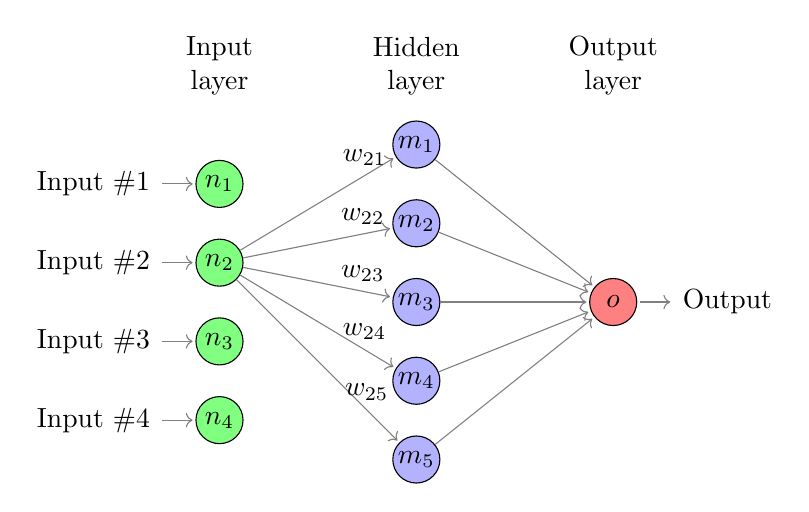
\begin{tikzpicture}[shorten >=1pt,->,draw=black!50, node distance=\layersep]
%https://tex.stackexchange.com/questions/96846/how-to-place-label-in-middle-of-line-above-and-below-with-tikz
    \tikzstyle{every pin edge}=[<-,shorten <=1pt]
    \tikzstyle{neuron}=[circle,fill=black!25,minimum size=17pt,inner sep=0pt, draw=black]
    \tikzstyle{input neuron}=[neuron, fill=green!50];
    \tikzstyle{output neuron}=[neuron, fill=red!50];
    \tikzstyle{hidden neuron}=[neuron, fill=blue!30];
    \tikzstyle{annot} = [text width=4em, text centered]

    % Draw the input layer nodes
    \foreach \name / \y in {1,...,4}
    % This is the same as writing \foreach \name / \y in {1/1,2/2,3/3,4/4}
        \node[input neuron, pin=left:Input \#\y] (I-\name) at (0,-\y) {$n_\y$};

    % Draw the hidden layer nodes
    \foreach \name / \y in {1,...,5}
        \path[yshift=0.5cm]
            node[hidden neuron] (H-\name) at (\layersep,-\y cm) {$m_\y$};

    % Draw the output layer node
    \node[output neuron,pin={[pin edge={->}]right:Output}, right of=H-3] (O) {$o$};

    % Connect every node in the input layer with every node in the
    % hidden layer.
%    \foreach \source in {1,...,4}
%        \foreach \dest in {1,...,5}
%            \draw (I-\source) -- node[below] {$w_ij$} ++ (H-\dest);


%    \foreach \source in {1,...,4}
        \foreach \dest in {1,...,5}
            \draw (I-2) -- node[above, pos=0.8] {$w_{2\dest}$} ++ (H-\dest);

    % Connect every node in the hidden layer with the output layer
    \foreach \source in {1,...,5}
        \path (H-\source) edge (O);

    % Annotate the layers
    \node[annot,above of=H-1, node distance=1cm] (hl) {Hidden layer};
    \node[annot,left of=hl] {Input layer};
    \node[annot,right of=hl] {Output layer};
\end{tikzpicture}
  \end{minipage}
  \vfill
\begin{minipage}[t][0.5\textheight][t]{\textwidth}

\end{minipage}


\end{frame}




\begin{frame}[fragile]{Point Variance of Linear Predictor}

\begin{align*}
\action<+->{ &=&&}
\\
\action<+->{  &=   && }
\end{align*}
\action<+->{The}
\end{frame}



\begin{frame}[fragile]{Correlation}
\begin{itemize}
\item[] \textbf{Serial No.} is basically uncorrelated with anything. \pause
\item[] \textbf{Admit} is highly correlated with \textbf{CGPA}, \textbf{TOEFL Score} and \textbf{GRE Score}\pause
\item[] \textbf{Research} has a lowish correlation with \textbf{Admit}, but also with everything else.  
\end{itemize}
\end{frame}











\begin{frame}[fragile]{Bias, Variance and Parameters}
  \begin{minipage}[t][0.5\textheight][t]{\textwidth}
	\centering
	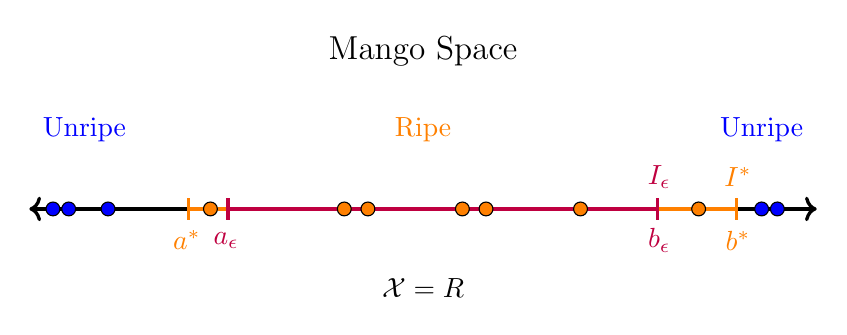
\begin{tikzpicture}
		\draw[<->,very thick] (-5,0) -- (5,0);
		\draw[color = orange, |-|,very thick] (-3,0) -- (4,0);
		\node[color=orange] at (4,.4) {$I^*$};
		\node at (0,2) {\large Mango Space} ;
		\node at (0,-1) {$\mathcal{X} = \mathbb{R}$} ;
		\node [color=blue] at (-4.3,1) {Unripe} ;
		\node [color=blue] at (4.3,1) {Unripe} ;
		\node [color=orange] at (0,1) {Ripe} ;

		\node [color=orange] at (-3,-.4) {$a^*$} ;
		\node [color=orange] at (4,-.4) {$b^*$} ;

		\draw [color=purple, |-|,very thick] (-2.5,0) -- (3,0);
		\node [color=purple] at (3,.4) {$I_\epsilon$} ;
		\node [color=purple] at (-2.5,-.4) {$a_\epsilon$} ;
		\node [color=purple] at (3,-.4) {$b_\epsilon$} ;

%		\draw [color=olive, |-|,very thick] (-3.5,0) -- (2.5,0);
%		\node [color=olive] at (3,.4) {$h_{\mathcal{T}}$} ;



		\node[circle,draw=black, fill=orange, inner sep=0pt,minimum size=5pt] at (2,0) {};
		\node[circle,draw=black, fill=orange, inner sep=0pt,minimum size=5pt] at (-1,0) {};
		\node[circle,draw=black, fill=orange, inner sep=0pt,minimum size=5pt] at (-.7,0) {};
		\node[circle,draw=black, fill=orange, inner sep=0pt,minimum size=5pt] at (.5,0) {};
		\node[circle,draw=black, fill=orange, inner sep=0pt,minimum size=5pt] at (.8,0) {};
		\node[circle,draw=black, fill=orange, inner sep=0pt,minimum size=5pt] at (-2.7,0) {};
		\node[circle,draw=black, fill=orange, inner sep=0pt,minimum size=5pt] at (3.5,0) {};

		\node[circle,draw=black, fill=blue, inner sep=0pt,minimum size=5pt] at (-4.5,0) {};
		\node[circle,draw=black, fill=blue, inner sep=0pt,minimum size=5pt] at (-4,0) {};
		\node[circle,draw=black, fill=blue, inner sep=0pt,minimum size=5pt] at (-4.7,0) {};
		\node[circle,draw=black, fill=blue, inner sep=0pt,minimum size=5pt] at (4.3,0) {};
		\node[circle,draw=black, fill=blue, inner sep=0pt,minimum size=5pt] at (4.5,0) {};
	\end{tikzpicture}
  \end{minipage}
  \vfill
  \begin{minipage}[t][0.5\textheight][t]{\textwidth}
Lets understand this visually.
$$
Err(x_0) = \sigma_\epsilon^2 + [E_\cT[\hat f(x_0)] - f(x_0)]^2 + E_\cT\big[ \hat{f}(x_0) - E_\cT[\hat{f}(x_0)] \big]^2\,.
$$\pause
Consider a data set, 
\end{minipage}
\end{frame}





























